\section{Расчет биологической защиты} %TODO: убрать для репорта
\subsection{Постановка задачи}
Необходимо рассчитать дозу облучения при стационарном режиме работы ЯЭУ ВВЭР-1000 за биологической защитой

\subsection{Построение расчетной модели биологической защиты}
Для формирования расчетной модели рассмотрим разомкнутую компоновку элементов и помещений ЯЭУ с РУ ВВЭР-1000. Такая компоновка предполагает разделения реакторного и машинного залов в разные здания, что позволяет локализовать возможную аварию и обеспечить большую безопасность.

\begin{figure}[H]
	\begin{center}
		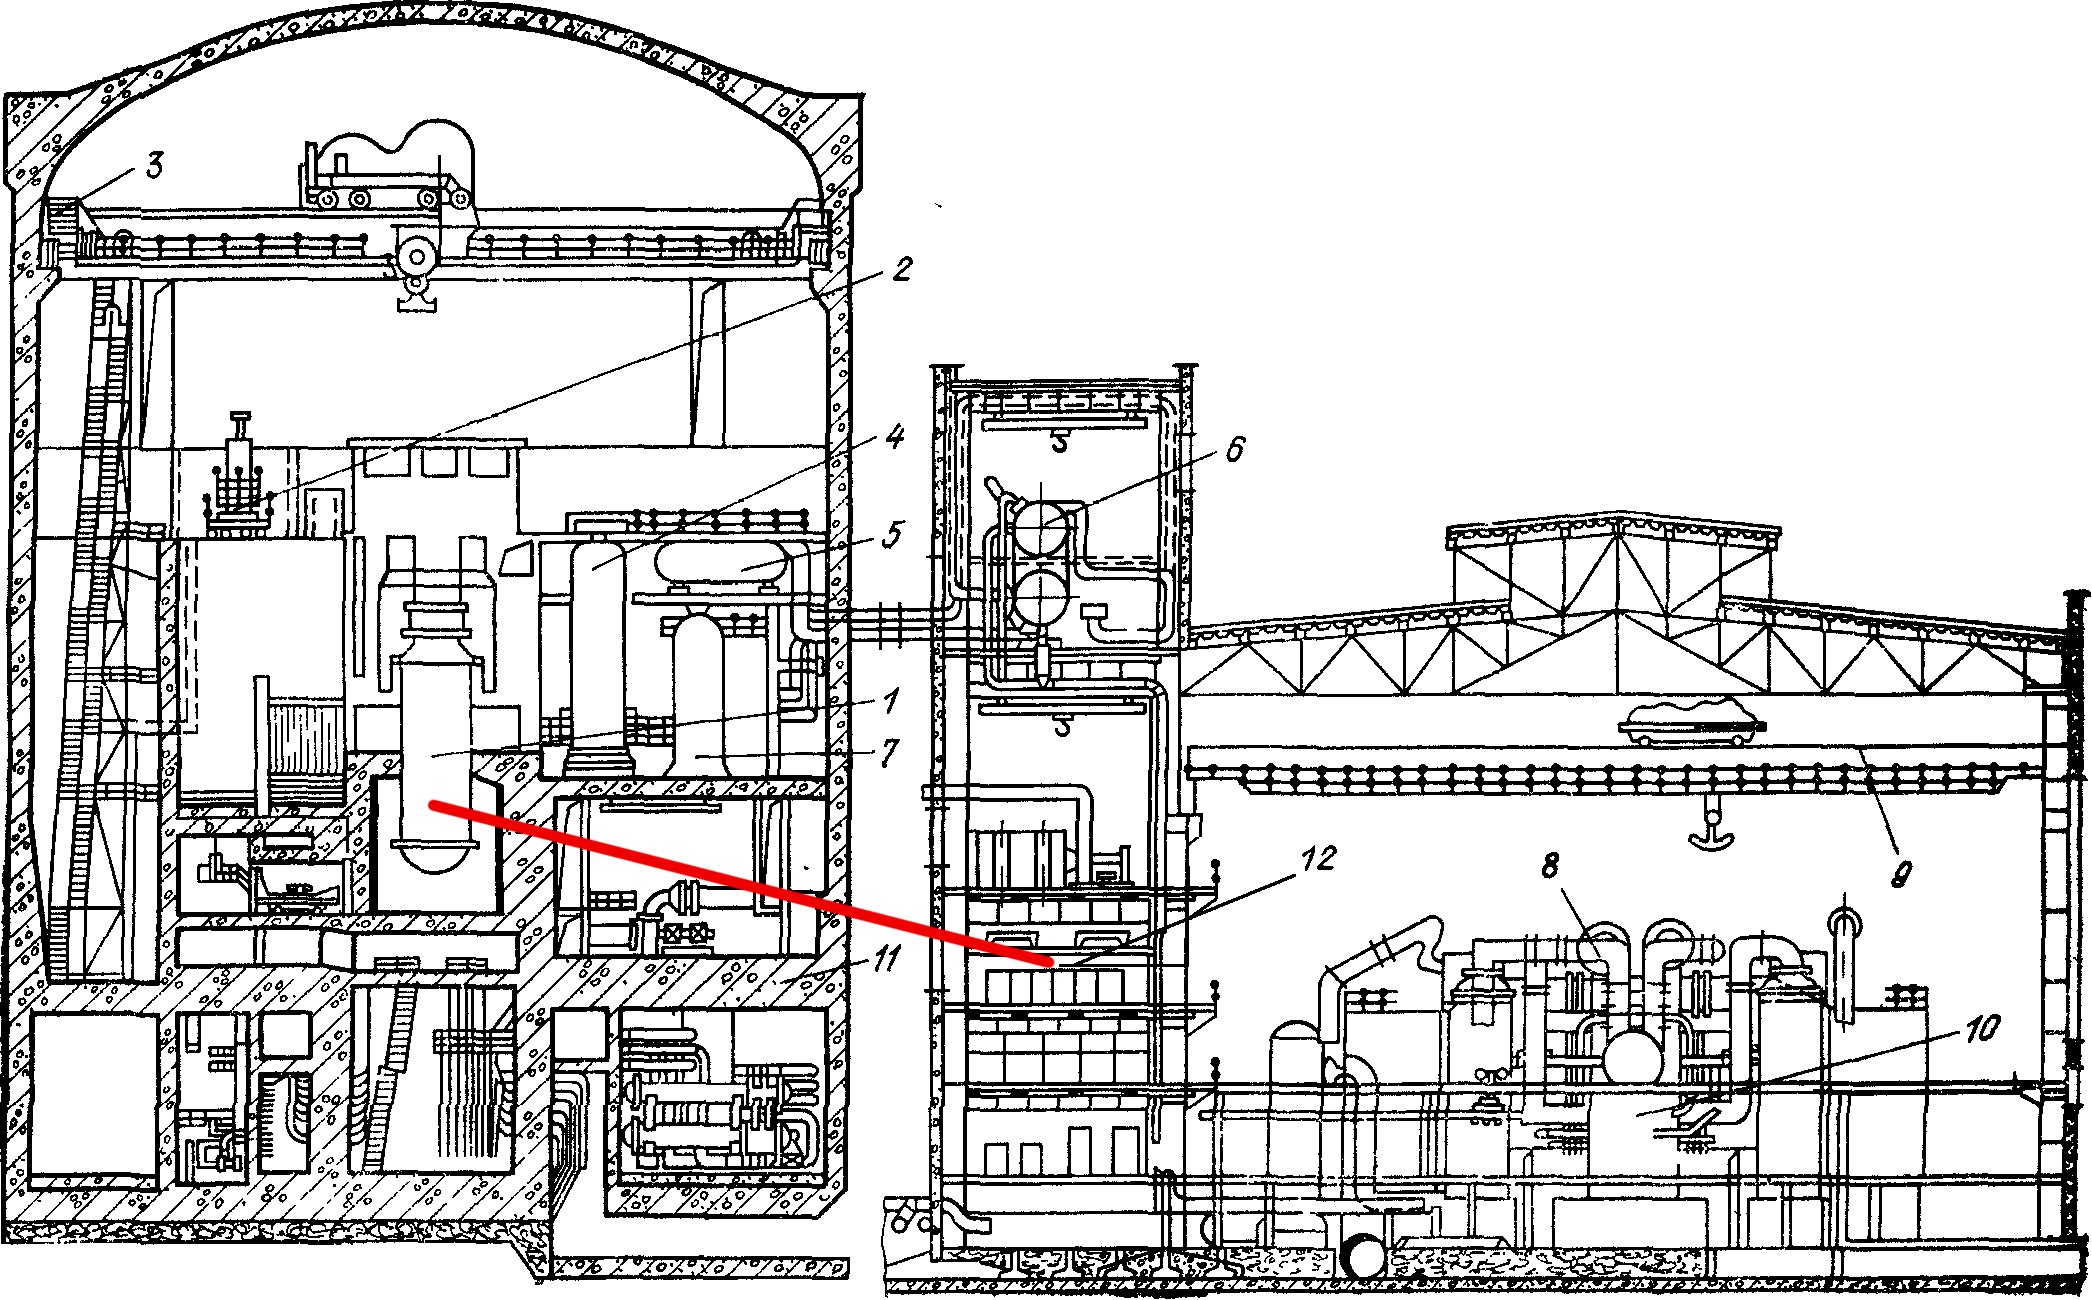
\includegraphics{razrez_bio.png}
		\caption{
			Общая компоновка энергоблока с РУ ВВЭР-1000 разомкнутой компоновки (Южно-Украинская АЭС) \cite{МонаховА.С1986Аэси}: \\
			1 — реактор; 2 — машина для перегрузки топлива; 3 — подъемный кран реакторного отделения; 4 — компенсатор давления, 5 — барботер; 6 — деаэратор; 7 — гидроемкость, 8 — турбогенератор; 9 — подъемный кран машинного зала; 10 — регенеративные подогреватели; 11 — защитная оболочка; 12 — блочный щит управления;
		}
		\label{pic:razrez_bio} % название для ссылок внутри кода
	\end{center}
\end{figure}
% Монахов Атомные электрические станции и их технологическое оборудование

\paragraph{Элементы компоновки вокруг реактора}

Рассмотрим основные элементы защиты, внешние по отношению к ВВЭР-1000 в сборе. Корпус реактора установливается в \textit{бетонную шахту} (рис \ref{pic:beton_shakhta}), которая играет роль основной опоры и крепления реактора с учетом сейсмических нагрузкок, а также биологической защиты от излучения со стороны АЗ. Между корпусом реактора и шахтой имеется кольцевой зазор, предназначенный для периодического контроля металла корпуса в связи с требованиями правил. Шахта резделена по высоте на два объема разделительным сильфоном: 
\begin{itemize}
	\item Верхний, снабжен гидрозатвором и соединяется с бассейном выдержки. При перегрузке верхний объем шахты вместе с бассейном заливается водой.
	\item Нижний, условно разделяемый фермой опорной на шахту зоны патрубков и шахту цилиндрической части корпуса. Соединяется проемом, снабженным герметичной дверью, с помещением для машины осмотра корпуса.
\end{itemize}
В помещении зоны патрубков
биологическая защита выполнена из металлических коробов, заполненных специальным составом, в который входят серпентинитовая галя, кристаллический карбид бора, дробь чугунная литая. В районе активной зоны применяется «сухая» защита, которая представляет из себя слой серпентинитового бетона толщиной
720 мм и высотой 4,7 м, облицованного металлической оболочкой. Такой бетон обладает высокой радиационной стойкостью, что позволяет удовлетворить требования по нейтронной защите. \cite{лескин2011физические}

\begin{figure}[H]
	\begin{center}
		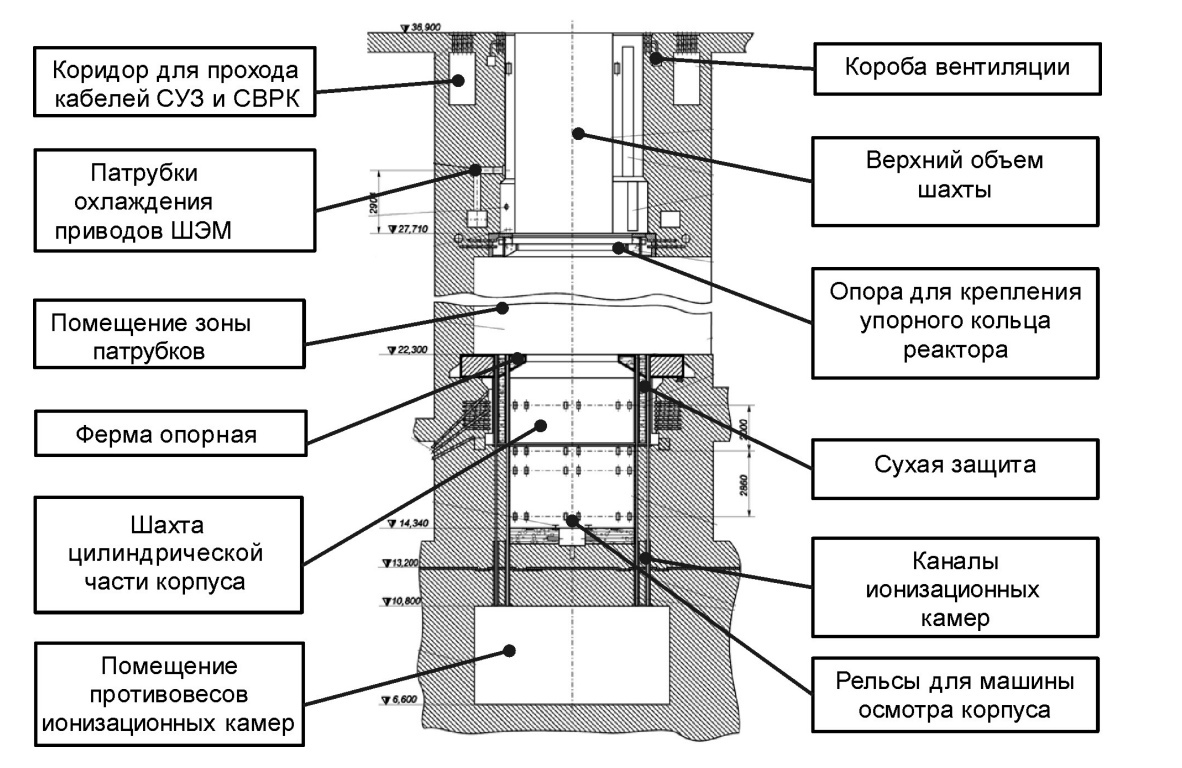
\includegraphics[scale=0.4]{beton.jpg}
		\caption{
			Бетонная шахта реактора 
		}
		\label{pic:beton_shakhta} % название для ссылок внутри кода
	\end{center}
\end{figure}

Все оборудование первого контура заключено в цилиндрическую оболочку, в верхней части которой расположен грузоподъемный поворотный кран. Между реакторным и машинным залами располагается этажерка электротехнических устройств, где размещены также деаэраторы и различные лаборатории.

\paragraph{Корпус и внутрикорпусные элементы компоновки} Корпус представляет собой вертикальный герметичный сосуд
цилиндрической формы с эллиптическими днищем и крышкой  с наружним диаметром 4535 мм, высотой 10.897 м и толщиной 192 мм в цилиндрической части и 210 мм в районе патрубков \cite{лескин2011физические}. В качестве основного материала используется сталь сталь 15Х2НМФА. е. Вся внутренняя поверхность корпуса покрыта
антикоррозионной наплавкой из нержавеющей стали толщиной не
менее 8 мм. В местах соприкосновения корпуса с крышкой, шахтой, уплотнительными прокладками, в местах приварки
кронштейнов, деталей крепления трубок КИП, на поверхности разделительного кольца выполнена наплавка толщиной не менее
15 мм. Внутрь реактора также устанавливается шахта, которая  представляет собой цилиндрическую обечайку с фланцем и эллиптическим днищем, в котором закреплены 163 опорные
трубы (стаканы) с шагом 236 мм, верхние части которых образуют
опорную плиту для установки и дистанционирования кассет активной зоны. Материал шахты – сталь 08Х18Н10Т толщиной 55 мм.

\paragraph{Устройство твэла} Твэл ядерного реактора ВВЭР-1000 представляет собой трубку, заполненную таблетками из двуокиси урана UO2 и герметично уплотненную концевыми деталями на сварке. Трубка твэла изготовлена из циркония, легированного 1 \% ниобия. Наружный диаметр трубки твэла 9.1±0.05 мм, ее толщина 0.65±0.03 мм, а внутренний диаметр 7.72+0.08 мм.
В эту трубку с зазором 0.19–0.32 мм на диаметр помещены таблетки двуокиси урана высотой (длиной) 20 мм и диаметром 7.57±0.04 мм. В середине этих таблеток имеются отверстия диаметром 1.5 мм, а края таблеток скруглены фасками. Общая длина столба этих таблеток в твэле составляет 3530 мм. Все размеры указаны для холодного состояния. Длина трубки твэла составляет 3800 мм, поэтому положение столба топливных таблеток в твэле зафиксировано разрезными втулками из нержавеющей стали и пружиной, не препятствующими тепловым перемещениям. Вид твэла приведён на рис. \ref{pic:tvel} \cite{ТвэлТерновых}

\begin{figure}[H]
    \begin{center}
        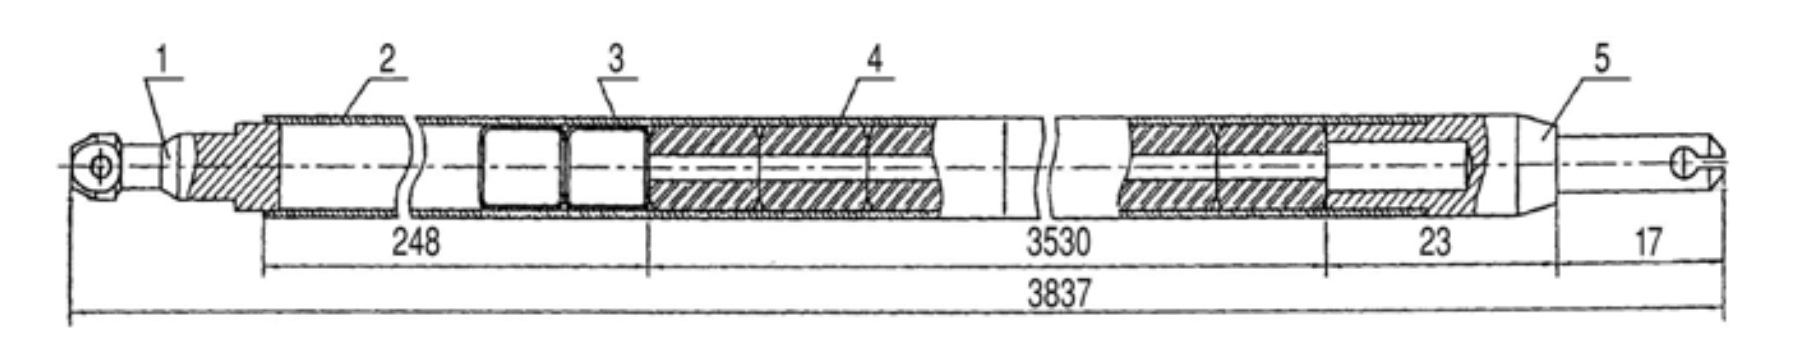
\includegraphics[scale=0.3]{tvel.jpg}
        \caption{
                Тепловыделяющий элемент: 1 – заглушка верхняя; 2 – оболочка; 3 – фиксатор; 4 – таблетка; 5 – заглушка нижняя
        }
        \label{pic:tvel}
    \end{center}
\end{figure}

Преимущество циркония заключается в удачном сочетании ядерных и физических характеристик с механическими и коррозионными свойствами. Цирконий коррозионно стоек в большинстве сред, применяемых в качестве теплоносителей ядерных реакторов, и достаточно технологичен.

Естественная радиоактивность одной свежей ТВС составляет $1.8 \cdot 10^{10}$ Бк., гамма- излучение на поверхности около 0.2 бэр/ч.


\paragraph{Построение одномерной модели} В качестве помещения постоянного пребывания персонала рассматривается блочный щит управления, расположенный в этажерке электроустройств (цифра 12 на рис. \ref{pic:obsh}). Также в этажерке электроустройств размещаются распределительные устройства сетей электропитания двигателей электростанции, аккумуляторные батареи, трансформаторы и т. д.
Для построения расчетной модели был определен ряд значимых элементов конструкции реакторной установки с точки зрения нейтронной защиты. От активной зоны рассматриваемое помещение отделено внутрикорпусными элементами, такими как оболочка твэла, внутрикорпусная шахта; корпусом, бетонной внешней шахтой, внешней бетонной оболочкой реактора и бетонной стеной машинного зала. Суммарный слой бетона складывается из 3 м основания гермооболочки, 0.72 м сухой защиты шахты, 1.5 м шахты и 0.5 м стены машинного зала перед этажеркой.
Основная доля нейтронного излучения в реакторе приходится на нейтроны теплового спектра. Для таких энергий хрошими поглотителями являются кадмий, графит, бетон. 
Присутствующее гамма-излучение для своего эффективного поглощения требует свинец и подобные высокоплотные материалы. Таким образом были выбран слои биологической защиты, представленные в таблице \ref{tabular:bio-sec-layers}:

\begin{table}[H]
	\caption{Слои биологической защиты}
	\begin{center}
        \begin{tabular}{|l|c|c|c|}
        \toprule
         Название & Материал & Размер, см & Плотность, $\text{г}/\text{см}^3$ \\ 
         \midrule
         \hline
         Внутрикорпусная шахта & сталь 08Х18Н10Т & 5.5 & 7.9 \\
         \hline
         Теплоноситель & $\text{H}_2\text{O}$ & 26.3 & 0.71\\
         \hline
         Корпус & сталь 15Х2НМФА & 19.25 & 7.8 \\
         \hline
         Шахта + гермооболочка + стена & бетон & 572 & 2.35 \\
         %\hline
         %Герметичная оболочка & бетон &  & 2.5 \\ 
         \bottomrule
		\end{tabular}
		\label{tabular:bio-sec-layers}
	\end{center}
\end{table}

\subsection{Расчет дозы нейтронов из активной зоны реактора}


\begin{table}[H]
	\caption{Основные параметры для расчета}
	\begin{center}
        \begin{tabular}{|l|c|}
        \toprule
         Параметр & Значение \\ 
         \midrule
         \hline
         Тепловая мощность реактора, МВт $W_{\text{теп}}$ & $2.904 \cdot 10^3$ \\ 
         \hline
         Средняя энергия, выделяющаяся в одной реакции деления, МэВ $E_f$ & 200  \\ 
         \hline
         Средняя энергия нейтронов спектра деления, МэВ $E_{nf}$ & 2 \\
         \hline
         Среднее число нейтронов деления на середину кампани, $\nu_f$ & 2.42 \\
         \hline
         Коэффициент размножения $K_\infty$ & 1.03  \\
         \hline
         Доля нейтронов спектра деления в спектре утечки $\gamma$ & 0.5 \\
         \hline
         Среднее число гамма-квантов деления на середину кампании & 7.51 \\
         \hline
         Высота активной зоны $H_{\text{аз}}$, м & 3.5 \\
         \hline
         Радиус активной зоны $R_{\text{аз}}$, м & 1.58 \\
         \bottomrule
		\end{tabular}
		\label{tabular:bio_sec_in}
	\end{center}
\end{table}


\noindent Число реакций деления в реакторе в единицу времени:
\begin{equation}
        N_f = \frac
               { W_{ \text{теп} } }
        %   -------------------------
                   { E_f  }
\end{equation}
$$
       N_f = \frac
                     { 2.90 \cdot 10^{{ 9 }} }
 %   -------------------------------------------------------
    { 2.00 \cdot 10^{{ 2 }} \cdot 1.60 \cdot 10^{{ -13 }} }
= 9.06 \cdot 10^{{ 19 }}
\ \frac{\text{дел} } {\text{с} }
$$

\noindent Число нейтронов, образующихся в реакторе в единцу времени:
\begin{equation}
        N_n = N_f \cdot \nu_f
\end{equation}
$$
        N_n = 9.06 \cdot 10^{{ 19 }} \cdot 2.42  = 2.19 \cdot 10^{{ 20 }} \ \frac{нейтронов} {с}
$$

\noindent Площадь полной поверхности акивной зоны
\begin{equation}
        S_{\text{пов}} = S_{\text{бок}} + 2S_{\text{top}}
\end{equation}
\noindent где
\begin{itemize}
        \item $S_\text{бок} = H_{\text{аз}}2 \pi R_{\text{аз}}$
        \item $S_{\text{top}} = \pi R_{\text{аз}} ^ 2$
\end{itemize}
$$
        S_{\text{пов}} = 3.50  \cdot 2 \cdot \pi \cdot 1.58  + 2 \cdot \pi \cdot (1.58 )^2 = 5.04 \cdot 10^{{ 1 }}\ \text{м}^2
$$

\noindent Поток нейтронов утечки из активной зоны:
\begin{equation}
        \Phi = \frac
                   {N_n(K_\infty - 1)}
              % ------------------------
                   {S_{\text{пов}}}
\end{equation}
$$
        \Phi = \frac{2.19 \cdot 10^{{ 20 }} (1.03  - 1)} {5.04 \cdot 10^{{ 1 }}} = 1.30 \cdot 10^{{ 17 }}\ \frac{\text{нейтрон}}{\text{с} \cdot \text{м}^2}
$$

\noindent Поток нейтронов спектра деления в утечке из активной зоны:
\begin{equation}
        \Phi_f = \Phi \cdot \gamma
\end{equation}
$$
        \Phi_f = 1.30 \cdot 10^{{ 17 }} \cdot 5.00 \cdot 10^{{ -01 }} = 6.52 \cdot 10^{{ 16 }}\ \frac{\text{нейтрон}} {\text{с} \cdot \text{м}^2}
$$

\noindent Мощность экивалентной дозы нейтронов перед защитой
\begin{equation}
        D_{0n} = \Phi_f \cdot E_{nf} \cdot \overline{\mu_{\text{ЭН}}} \cdot K 
\end{equation}
\noindent где
\begin{itemize}
        \item $\overline{\mu_{\text{ЭН}}} = \frac {1\ \text{м}^2} {100\ \text{кг}}$ — массовый коэффициент поглощения энергии в биологической ткани, принимается равным отношению площади человека к его массе
        \item $K = 10\ \frac {\text{Зв}}{\text{Гр}}$ — коэффициент качества нейтронов спектра деления
\end{itemize}
$$
        D_{0n} = 6.52 \cdot 10^{{ 16 }} \cdot 2.00  \cdot 1.60 \cdot 10^{{ -13 }} \cdot 1.00 \cdot 10^{{ -02 }} \cdot 1.00 \cdot 10^{{ 1 }} = 2.09 \cdot 10^{{ 3 }}\ \frac{\text{Зв}}{\text{c}}
$$
Результаты расчетов дозы нейтронов из активной зоны представлены в таблице \ref{tabular:bio_sec_1_out}

\begin{table}[H]
	\caption{Результаты расчета дозы нейтронов}
	\begin{center}
        \begin{tabular}{|l|c|}
        \toprule
         Параметр & Значение \\
         \midrule
         \hline
         $N_f$, $\frac{\text{дел}}{\text{с}}$ & $9.06 \cdot 10^{19}$ \\ 
         \hline
         $N_n$, $\frac{\text{нейтрон}}{\text{с}}$ & $2.19 \cdot 10^{20}$ \\
         \hline
         $S_{\text{пов}}$, $\text{м}^2$ & $50.4$ \\
         \hline
         $\Phi, \frac{\text{нейтрон}}{\text{м}^2 \cdot \text{с}}$ & $1.3 \cdot 10^{17}$\\
         \hline
         $\Phi_f, \frac{\text{нейтрон}}{\text{м}^2 \cdot \text{с}}$ & $6.52 \cdot 10^{16}$ \\
         \hline
         $D_{0n}, \frac{\text{Зв}}{\text{с}}$ & $2.09 \cdot 10^3$ \\
         \bottomrule
		\end{tabular}
		\label{tabular:bio_sec_1_out}
	\end{center}
\end{table}


\subsection{Расчет дозы нейтронов за защитой или минимального размера слоя биологической защиты для нейтронов}
Для расчета дозы нейтронов за защитой используется модель сечения выведения многослойной системы.

\noindent Сечение выведение для многослойной системы:

\begin{equation}
        D = D_0 \exp\left(
                - \sum_i \Sigma_{\text{rem}}^i \cdot d_i
        \right)
\end{equation}

\noindent Для текущей модели раскрывается как:

\begin{equation}
        D = D_0 \exp\left(
                - \Sigma_{\text{rem}}^{\text{H}_2\text{O}} \cdot d_{\text{H}_2\text{O}}
                - \Sigma_{\text{rem}}^{\text{ст}} \cdot d_{\text{ст}}
                - \Sigma_{\text{rem}}^{\text{ж/б}} \cdot d_{\text{ж/б}}
        \right)
\end{equation}
\noindent где $\Sigma_{\text{rem}}^{\text{H}_2\text{O}}$ — сечение выведеня слоя воды,
              $\Sigma_{\text{rem}}^{\text{ст}}$ — сечение выведения слоя стали,
              $\Sigma_{\text{rem}}^{\text{ж/б}}$ — сечение выведения слоя бетона,
              $d_{\text{H}_2\text{O}}, d_{\text{ст}}, d_{\text{ж/б}}$ — толщины слоев воды, стали и бетона


\begin{table}[H]
	\caption{Значения сечений выведений защиты и толщины различных слоев \cite{ТвэлТерновых}}
	\begin{center}
        \begin{tabular}{|l|c|c|c|}
        \toprule
         Слой защиты & d, см & $\rho, \frac{\text{г}}{\text{см}^3}$ & $\Sigma_{\text{rem}}$, $\text{см}^{-1}$\ \\
         \midrule
         \hline
         Вода & 26.3 & 0.71 & 0.069 \\
         \hline
         Сталь & 24.75 & 7.9 & 0.166 \\
         \hline
         Бетон & 572 & 2.35 & 0.08 \\
         \bottomrule
		\end{tabular}
		\label{tabular:bio_sec_2_in}
	\end{center}
\end{table}
% TODO: все формулы в equation, числовые выражения -- в далары
$$
        D_n = 2.09 \cdot 10^{{ 3 }} \exp\left( 
                -6.90 \cdot 10^{{ -02 }}\cdot2.63 \cdot 10^{{ 1 }}
                -1.66 \cdot 10^{{ -01 }}\cdot2.48 \cdot 10^{{ 1 }}
                -8.00 \cdot 10^{{ -02 }}\cdot5.72 \cdot 10^{{ 2 }}
        \right) = 7.49 \cdot 10^{{ -20 }}\ \frac{\text{Зв}}{\text{с}}
$$
\noindent Для учета 20\% погрешности по дозе модели сечения выведения необходимо использовать поправочный коэффициент 1.2. Итоговая доза с учетом погрешности в Зв / нед:
$$
        D_{n, \text{нед}} = 1.2 \cdot 7 \cdot 24 \cdot 60 \cdot 60 \cdot 7.490 \cdot 10^{{ -20 }} = 5.436 \cdot 10^{{ -14 }}\ \frac{\text{Зв}}{\text{нед}}
$$


\subsection{Расчет дозы гамма-квантов из активной зоны}
Для расчета гамма-квантов перед защитой применен приближенный алгоритм. Его идея – оценить поток гамма-квантов деления из активной зоны реактора в одномерной геометрии и внести поправку на утечку гамма-квантов от других их источников.

\noindent Число гамма-квантов, образующихся в реакторе в единицу времени: 
\begin{equation}
        I = N_f \cdot \nu_\gamma \cdot N_\gamma
\end{equation}
\noindent где $N\gamma$ — доля гамма-квантов определенной энергии в реакции деления, для
E=3 МэВ $N_{\gamma, 3 \text{МэВ}}=0.2$, для E=5 МэВ $N_{\gamma, 5 \text{МэВ}} = 0.15$
Тогда число гамма-квантов в единицу времени для двух энергий:
\begin{align*}
        I_{3\ \text{МэВ}} &= 9.064 \cdot 10^{{ 19 }} \cdot 2.000 \cdot 10^{{ -01 }} \cdot 7.510  = 1.361 \cdot 10^{{ 20 }}\ \frac{\text{кв}}{\text{с}} \\
        I_{5\ \text{МэВ}} &= 9.064 \cdot 10^{{ 19 }} \cdot 1.500 \cdot 10^{{ -01 }} \cdot 7.510  = 1.021 \cdot 10^{{ 20 }}\ \frac{\text{кв}}{\text{с}}
\end{align*}
Рассмотрим перенос нерассеянных гамма-квантов в однородной пластине с внешним источником, перпендикулярным границам пластины. При этом потребуем выполнения следующих условий:
\begin{enumerate}
        \item  толщина пластины равна $L$ – средней ходе активной зоны $L = \frac{4 V_{\text{аз}}}{S_{\text{пов}}}$, где $V_{\text{аз}}$ – объем активной зоны
        \item линейный коэффициент ослабления пластины $\mu_\gamma$ вычисляется через коэффициенты ослабления элементарной ячейки реактора
        \begin{equation}
                \mu_\gamma = \mu_U\varepsilon_U + \mu_{\text{об}}\varepsilon_{\text{об}}+\mu_{\text{т/н}}\varepsilon_{\text{т/н}} + \mu_{\text{зам}}\varepsilon_{\text{зам}}
        \end{equation}
        где $\varepsilon_i$ – объемные доли топлива, конструкционных материалов, теплоносителя и замедлителя в элементарной ячейке.
\end{enumerate}

\begin{table}[H]
	\caption{Объемные доли материалов}
	\begin{center}
        \begin{tabular}{|l|c|}
        \toprule
         Материал & Обьемная доля $\varepsilon_i$ \\
         \midrule
         \hline
         Топливо & 0.166 \\
         \hline
         Оболочка (Zr) & 0.071 \\
         \hline
         теплоноситель/замедлитель (вода) & 0.733 \\
         \bottomrule
		\end{tabular}
		\label{tabular:objem_doli}
	\end{center}
\end{table}

\begin{table}[H]
	\caption{Линейные коэффициенты ослабления $\mu$ для гамма-квантов с энергией 3 и 5 МэВ}
	\begin{center}
        \begin{tabular}{|l|c|c|}
        \toprule
         Материал & $\mu_3, \text{см}^{-1}$ & $\mu_5, \text{см}^{-1}$ \\
         \midrule
         \hline
         Топливо & 0.81 & 0.83 \\
         \hline
         Оболочка (Zr) & 0.237 & 0.221\\
         \hline
         теплоноситель/замедлитель (вода) & 0.028 & 0.021\\
         \bottomrule
		\end{tabular}
		\label{tabular:koeff_oslab}
	\end{center}
\end{table}
\noindent Таким образом полный линейный коэффициент ослабления для энергий E=3 МэВ, 5 Мэв:
\begin{align*}
        \mu_{\gamma, 3\ \text{Мэв}} &= 1.66 \cdot 10^{{ -1 }}\cdot8.10 \cdot 10^{{ -1 }} + 7.10 \cdot 10^{{ -2 }}\cdot2.37 \cdot 10^{{ -1 }} + 7.33 \cdot 10^{{ -1 }}\cdot2.80 \cdot 10^{{ -2 }}\\ &= 1.72 \cdot 10^{{ -1 }}\ \text{см}^{-1} \\
\\
    \mu_{\gamma, 5\ \text{Мэв}} &= 1.66 \cdot 10^{{ -1 }}\cdot8.30 \cdot 10^{{ -1 }} + 7.10 \cdot 10^{{ -2 }}\cdot2.21 \cdot 10^{{ -1 }} + 7.33 \cdot 10^{{ -1 }}\cdot2.10 \cdot 10^{{ -2 }} \\&= 1.69 \cdot 10^{{ -1 }}\ \text{см}^{-1}
\end{align*}
\noindent Объем активной зоны:
$$
V_{\text{аз}} = \pi R_{\text{аз}}^2 H_{\text{аз}} = \pi \cdot 1.58 ^ 2 \cdot 3.5 ^ 2 = 27.45 \text{м}^3
$$

\noindent Толщина пластины:
$$
L = \frac{4 \cdot 27.45} {5.04 \cdot 10^1} = 2.18 \text{м} = 217.7 \text{см}
$$
\noindent Источник гамма-квантов, равномерно распределенный по объему пластины:
\begin{equation}
        Q = \frac I L
\end{equation}
\begin{align*}
        Q_{3\ \text{Мэв}} = \frac{1.361 \cdot 10^{{ 20 }}}{2.177 \cdot 10^{{ 2 }}} = 6.253 \cdot 10^{{ 17 }} \frac{\text{кв}}{\text{с} \cdot \text{см}} \\
        Q_{5\ \text{Мэв}} = \frac{1.021 \cdot 10^{{ 20 }}}{2.177 \cdot 10^{{ 2 }}} = 4.690 \cdot 10^{{ 17 }} \frac{\text{кв}}{\text{с} \cdot \text{см}} \\
\end{align*}
\noindent Число нерассеянных гамма-квантов через поверхность пластины
\begin{equation}
        N = \frac{Q}{\mu_\gamma}\left(1 - \exp\left(-\mu_\gamma L\right)\right)
\end{equation}
\begin{align*}
        N_{3\ \text{МэВ}} = \frac{6.25 \cdot 10^{{ 17 }}}{1.72 \cdot 10^{{ -1 }}} \cdot \left( 1 - \exp\left(-1.72 \cdot 10^{{ -1 }}\cdot2.18 \cdot 10^{{ 2 }}\right)\right) = 3.64 \cdot 10^{{ 18 }} \frac{\text{кв}}{\text{с}} \\
        N_{5\ \text{МэВ}} = \frac{4.69 \cdot 10^{{ 17 }}}{1.69 \cdot 10^{{ -1 }}} \cdot \left( 1 - \exp\left(-1.69 \cdot 10^{{ -1 }}\cdot2.18 \cdot 10^{{ 2 }}\right)\right) = 2.78 \cdot 10^{{ 18 }} \frac{\text{кв}}{\text{с}}
\end{align*}
\noindent Поток нерассеянных гамма-квантов деления из активной зоны:
\begin{equation}
        \Phi_\gamma = \frac N {S_{\text{пов}}}
\end{equation}
\begin{align*}
        \Phi_{\gamma, 3\ \text{МэВ}} = \frac{3.64 \cdot 10^{{ 18 }}}{5.04 \cdot 10^{{ 5 }}}  = 7.22 \cdot 10^{{ 12 }} \frac{\text{кв}}{\text{см}^2 \cdot \text{с}} \\
        \Phi_{\gamma, 5\ \text{МэВ}} = \frac{2.78 \cdot 10^{{ 18 }}}{5.04 \cdot 10^{{ 5 }}}  = 5.51 \cdot 10^{{ 12 }} \frac{\text{кв}}{\text{см}^2 \cdot \text{с}} 
\end{align*}

\noindent Полный поток гама-квантов из активной зоны с учетом поправочного коэффициента $\xi=2$:
\begin{equation}
        \Phi_\gamma^{\text{full}} = \Phi_\gamma \xi
\end{equation}
\begin{align*}
        \Phi_{\gamma, 3\ \text{МэВ}}^{\text{full}} = 7.22 \cdot 10^{{ 12 }} \cdot 2  = 1.44 \cdot 10^{{ 13 }} \frac{\text{кв}}{\text{см}^2 \cdot \text{с}} \\
    \Phi_{\gamma, 5\ \text{МэВ}}^{\text{full}} = 5.51 \cdot 10^{{ 12 }} \cdot 2  = 1.10 \cdot 10^{{ 13 }} \frac{\text{кв}}{\text{см}^2 \cdot \text{с}} 
\end{align*}

\noindent Мощность эквивалентной дозы гамма-квантов перед защитой
\begin{equation}
        D_{0\gamma}=\Phi_\gamma^{\text{full}} \cdot E \cdot \overline{\mu_{\text{ЭН}}} \cdot K
\end{equation}
\begin{align*}
        D_{0\gamma, 3\ \text{МэВ}} = 1.44 \cdot 10^{{ 13 }} \cdot 3 \cdot 1.60 \cdot 10^{{ -13 }} \cdot 100 \cdot 1 = 6.94 \cdot 10^{{ 2 }}\ \frac{\text{Зв}}{\text{c}} \\
        D_{0\gamma, 5\ \text{МэВ}} = 1.10 \cdot 10^{{ 13 }} \cdot 5 \cdot 1.60 \cdot 10^{{ -13 }} \cdot 100 \cdot 1 = 8.82 \cdot 10^{{ 2 }}\ \frac{\text{Зв}}{\text{c}}
\end{align*}
Результат расчета дозы гамма квантов из активной зоны для энергий 3, 5 МэВ представлены в таблицах \ref{tabular:bio_sec_3_out_3}, \ref{tabular:bio_sec_3_out_5} соответственно.

\begin{table}[H]
	\caption{Результаты расчета дозы гамма-квантов энергии 3 МэВ}
	\begin{center}
        \begin{tabular}{|l|c|}
        \toprule
         Параметр & Значение \\
         \midrule
         \hline
         $I_3, \text{кв}{с}$ & $1.36 \cdot 10^{20}$ \\
         \hline
         $L$, см & 217.7 \\
         \hline
         $Q_3$, кв / (см $\cdot$ c)  & $6.25 \cdot 10^{17}$ \\
         \hline
         $\Phi_\gamma 3$, $\frac{\text{кв}}{\text{см}^2 \cdot \text{с}}$ & $7.22 \cdot 10^{12}$ \\
         \hline
         $N_3$, кв / c & $3.64 \cdot 10^{18}$ \\ 
         \hline
         $D_{0\gamma\ 3}$, Зв / c & 694\\
         \hline
         \bottomrule
		\end{tabular}
		\label{tabular:bio_sec_3_out_3}
	\end{center}
\end{table}

\begin{table}[H]
	\caption{Результаты расчета дозы гамма-квантов энергии 5 МэВ}
	\begin{center}
        \begin{tabular}{|l|c|}
        \toprule
         Параметр & Значение \\
         \midrule
         \hline
         $I_5, \text{кв}{с}$ & $1.02 \cdot 10^{20}$ \\
         \hline
         $L$, см & 217.7 \\
         \hline
         $Q_5$, кв / (см $\cdot$ c)  & $4.69 \cdot 10^{17}$ \\
         \hline
         $\Phi_\gamma 5$, $\frac{\text{кв}}{\text{см}^2 \cdot \text{с}}$ & $5.51 \cdot 10^{12}$ \\ 
         \hline
         $N_5$, кв / c & $2.78 \cdot 10^{18}$ \\ 
         \hline
         $D_{0\gamma\ 5}$, Зв / c & 882\\
         \hline
         \bottomrule
		\end{tabular}
		\label{tabular:bio_sec_3_out_5}
	\end{center}
\end{table}
\subsection{Расчет дозы гамма-квантов за защитой или минимального размера слоя биологической защиты для гамма-квантов}
Для расчета дозы гамма-квантов за защитой или минимального размера слоя биологической защиты для гамма-квантов примиенена модель дозовых факторов накоплений.
Эквивалентная дозы нерассеянных гамма-квантов:
\begin{equation}
        D_\gamma = D_{0\gamma}\exp\left(
                -\sum_i\mu_{\gamma i} d_i
        \right)
\end{equation}
\noindent где $\mu_{\gamma i}$ — линейный коэффициент ослабления i-го слоя, $d_i$ — толщина i-го слоя
\begin{table}[H]
	\caption{Линейные коэффициенты ослабления $\mu$ для гамма-квантов с энергией 3 и 5 МэВ за активной зоной}
	\begin{center}
        \begin{tabular}{|l|c|c|}
        \toprule
         Материал & $\mu_3, \text{см}^{-1}$ & $\mu_5, \text{см}^{-1}$ \\
         \midrule
         \hline
         Сталь & 0.3 & 0.25 \\
         \hline
         Бетон & 0.08 & 0.07\\
         \hline
         Вода & 0.028 & 0.021\\
         \bottomrule
		\end{tabular}
		\label{tabular:koeff_oslab_2}
	\end{center}
\end{table}
\begin{align*}
        D_{\gamma, \text{нерас}, 3\ \text{МэВ}} &= 6.94 \cdot 10^{{ 2 }} \cdot \exp (
                - 3.00 \cdot 10^{{ -1 }} \cdot 2.48 \cdot 10^{{ 1 }}
                - 8.00 \cdot 10^{{ -2 }} \cdot 5.72 \cdot 10^{{ 2 }}
                \\ &- 2.80 \cdot 10^{{ -2 }} \cdot 2.63 \cdot 10^{{ 1 }}
        ) = 2.65 \cdot 10^{{ -21 }}\ \frac{\text{Зв} }{\text{с}} \\
        D_{\gamma, \text{нерас}, 5\ \text{МэВ}} &= 8.82 \cdot 10^{{ 2 }} \cdot \exp (
                - 2.50 \cdot 10^{{ -1 }} \cdot 2.48 \cdot 10^{{ 1 }}
                - 7.00 \cdot 10^{{ -2 }} \cdot 5.72 \cdot 10^{{ 2 }}
                \\ &- 2.10 \cdot 10^{{ -2 }} \cdot 2.63 \cdot 10^{{ 1 }}
        ) = 4.26 \cdot 10^{{ -18 }}\ \frac{\text{Зв} }{\text{с} }        
\end{align*}
Дозовый фактор, равный отношению эквивалентной дозы гамма-излучения для квантов всех энергий к эквивалентной дозе излучения нерасеянных гамма-квантов от одного источника
\begin{equation}
        B_D = \frac{D_{\text{нерас}} - D_{\text{рас}}}{D_{\text{нерас}}} = 1 + \frac{D_{\text{рас}}}{D_{\text{нерас}}}
\end{equation}
Тогда полная доза гамма-квантов за защитой:
\begin{equation}
        D_{\text{полн}} = B_D\cdot D_{\text{нерас}}
\end{equation}
Для нахождения фактора накоплени гомогенной среды можно применить формулу Тейлора:
\begin{equation}
        B(\mu d) = A_1\exp(-\alpha_1 \mu d) + (1 - A_1)\exp(- \alpha_2 \mu d)
\end{equation}
По формуле Д.Л. Бродлера:
\begin{equation}
        B_{ \text{гет} } =
        B_N \left( \sum_i^N \mu_i d_i \right)
        + \sum_{ n = 1 }^{ N - 1 } \left[
                B_n \left( \sum_i^n \mu_i d_i \right) 
                - B_{ n + 1 } \left( \sum_i^n \mu_i d_i3\right)
        \right]
\end{equation}
\noindent где $B_j \left( \sum_i^n\mu_i d_i \right)$ — фактор накопения, вычисляемые по формуле Тейлора. Тогда:
\begin{align*}
        B_{\text{гет}\ 3\ \text{МэВ}} &= 92.3 \\
        B_{\text{гет}\ 5\ \text{МэВ}} &= 34.7 \\
\end{align*}
\noindent Полная доза гамма-квантов за защитой:
\begin{align*}
        D_{\gamma\ 3\ \text{МэВ}} = 92.3 \cdot 2.65 \cdot 10^{ - 21}= 2.45 \cdot 10^{-19}\ \frac{\text{Зв}}{\text{с}}\\
        D_{\gamma\ 5\ \text{МэВ}} = 34.7 \cdot 4.26 \cdot 10^{ - 18}= 1.48 \cdot 10^{- 16 }\ \frac{\text{Зв}}{\text{с}}\\
\end{align*}
Мощность эквивалентной дозы, создаваемой гамма-квантами всех энергий за защитой в Зв / нед:
$$
D_\gamma = 7 \cdot 24 \cdot 60 \cdot 60 \cdot (D_{\gamma\ 3\ \text{МэВ}} + D_{\gamma\ 5\ \text{МэВ}}) = 8.95 \cdot 10^{ - 11 } \frac{\text{Зв}}{\text{нед}}
$$

Суммарная мощность, создаваемая за защитой нейтронами и гамма-квантами c учетом погрешности метода фактора накопления:
$$
D = 1.15(D_n + D_\gamma) = 1.15 \cdot (5.44 \cdot 10^{-14} + 8.95 \cdot 10^{-11}) = 1.03 
\cdot 10^{- 10}\ \text{Зв} / \text{нед}
$$

\subsection{Заключение}
В работе проводился расчет биологической защиты, была проведена оценка мощностей эквивалентных доз нейтронов и гамма-квантов за защитой.

Оценка проводилась для нейтронных потоков методом сечения выведения для системы со слоями, а также для гамма-квантов с энергиями 3 и 5 МэВ методом дозовых факторов накопления.

По результату работы было получена суммарная мощность эквивалентной дозы нейтронов и гамма-квантов за защитой не превышает $1.03 \cdot 10^{- 7} \frac{\text{мЗв}}{\text{нед}}$. Получившаяся доза сильно меньше предельной поглощенной дозы для персонала АЭС, которая составляет $0.4 \frac{\text{мЗв}}{\text{нед}}$, из чего можно сделать вывод, что рассматриваемое помещение БЩУ безопасно с точки зрения радиационной защиты

